To test the pipeline functionality was implemented that allows the user to select their own interferometer array layout and sky model. The user can then generate an image that that interferometer would see if it were to observe that sky model. If the image comes out similar to the sky model then the user knows the pipeline is working as intended. An example is given below: \\
Say the user were to select KAT7 as the interferometer and select this sky model: 
\begin{center}
    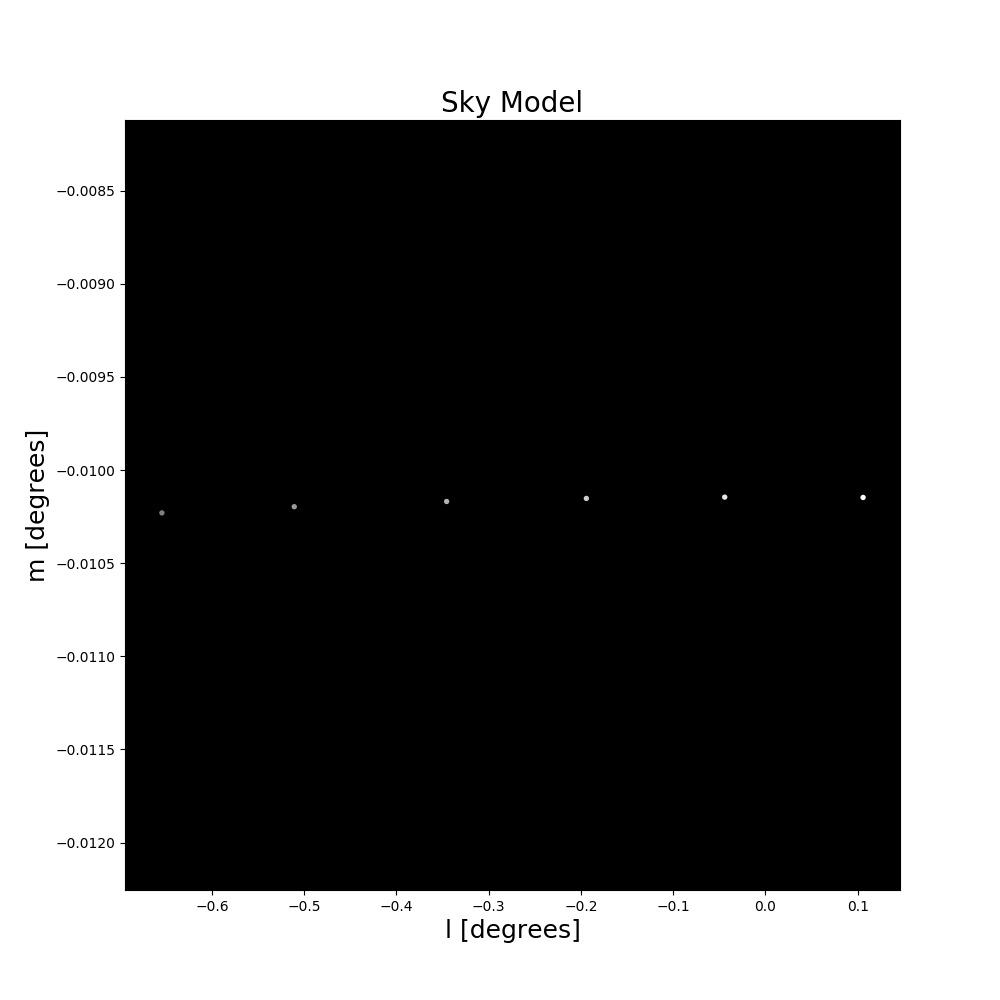
\includegraphics[scale=0.35]{images/SkyModel.png}
\end{center}
% \begin{figure}[h!]
%     \centering
%     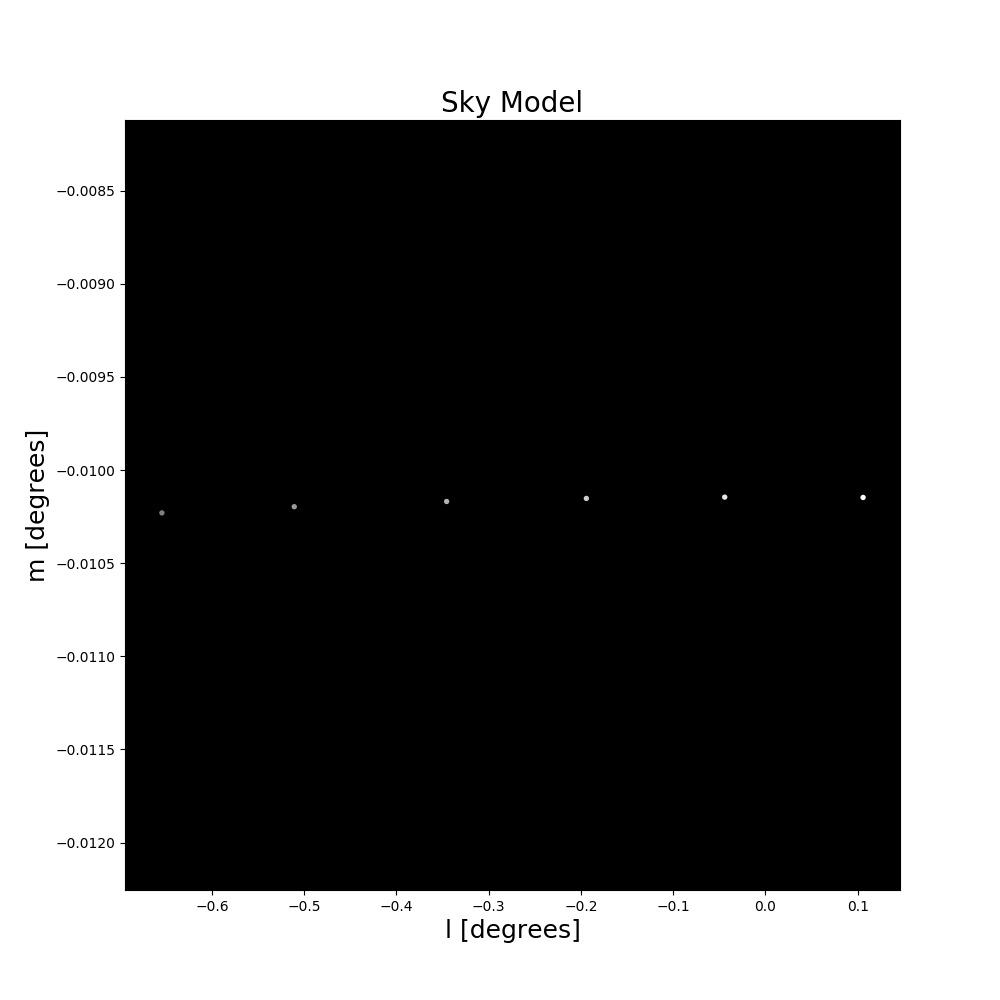
\includegraphics[scale=0.35]{images/SkyModel.png}
% \end{figure}
The testing framework will generate an image based off the interferometer and sky model, the output of this testing will be:
\begin{center}
    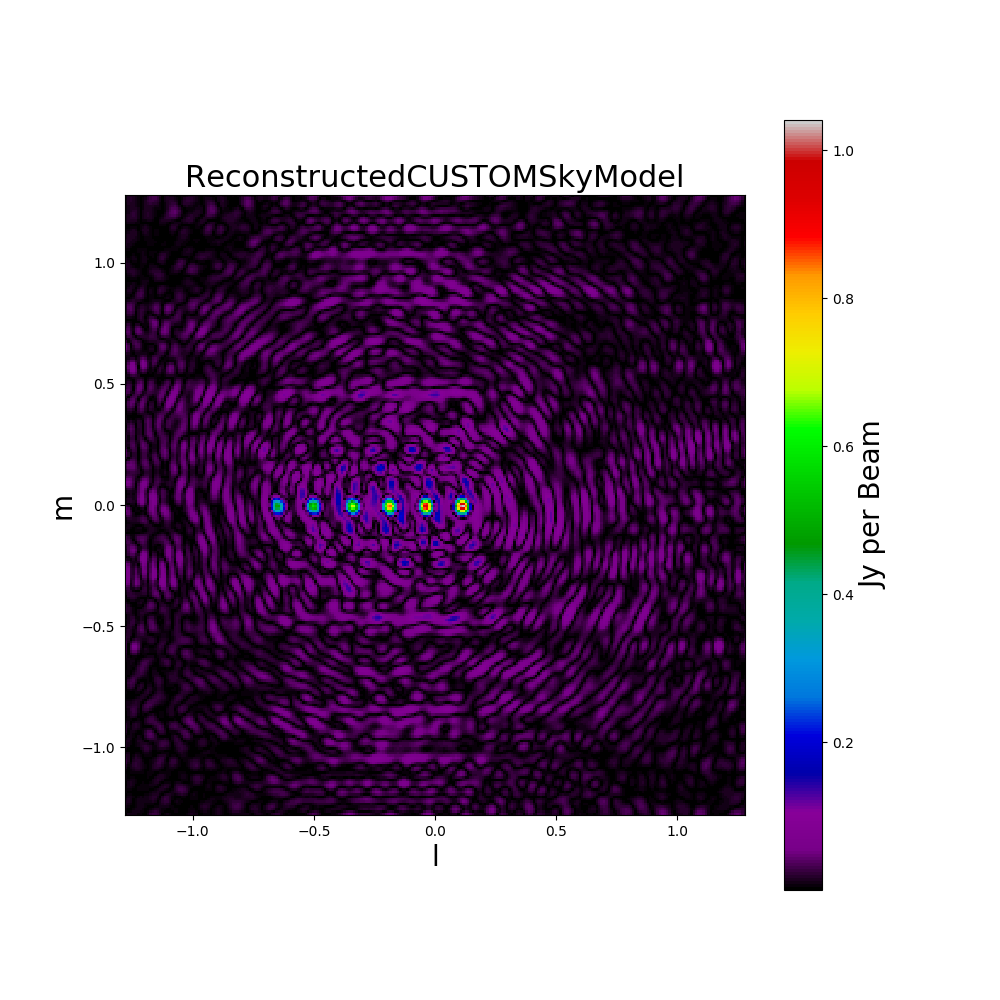
\includegraphics[scale=0.35]{images/ReconstructedCUSTOMSkyModel.png}
\end{center}
% \begin{figure}[h!]
%     \centering
%     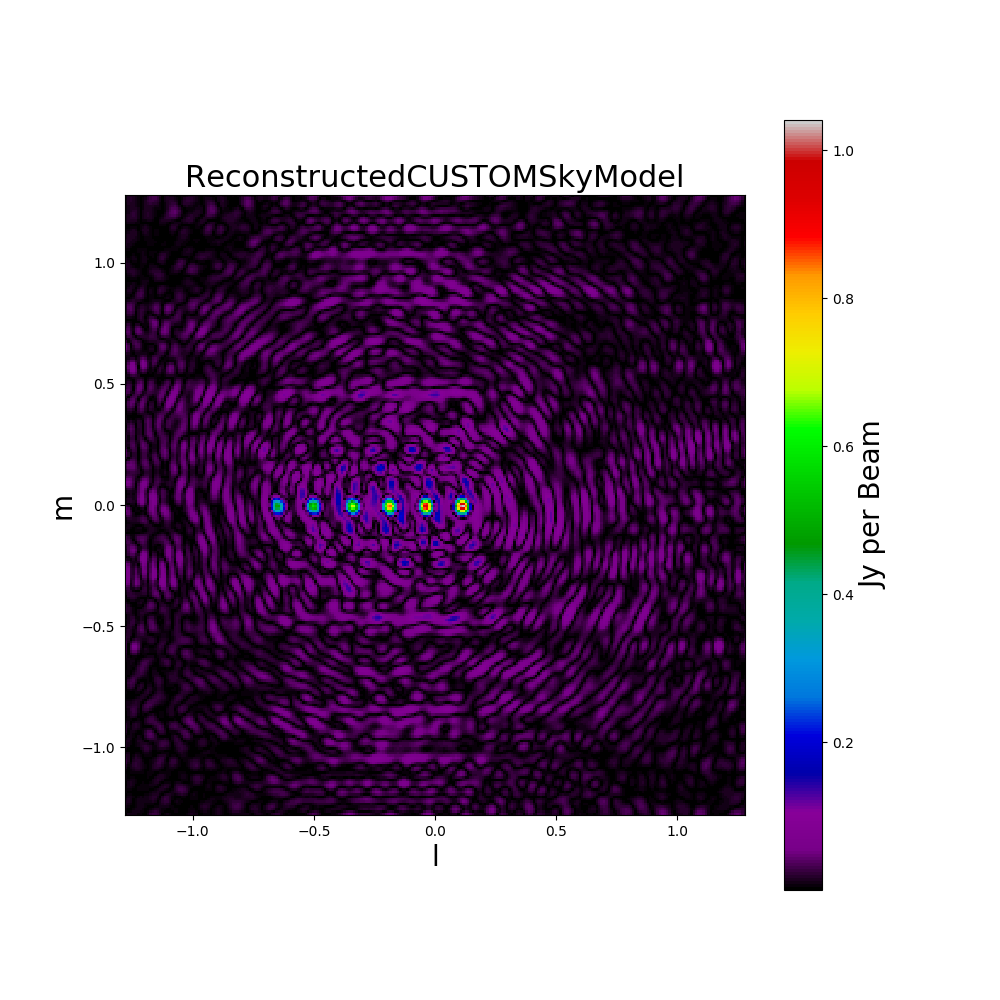
\includegraphics[scale=0.4]{images/ReconstructedCUSTOMSkyModel.png}
% \end{figure}
This experiment can be applied to many interferometers, real or imaginary with any sky model, and provided the cell size and resolution are chosen correctly, the testing framework will produce an image that closely resembles the original sky model.\\
This shows that the pipeline is working correctly and that the images that are created by the TART section are correct.
